% The Macro Transcension Hypothesis (Paper A) -- Swanson 2026
% arXiv-style single-column preprint. Self-contained: compile with
%   pdflatex macro-transcension-hypothesis.tex
%   pdflatex macro-transcension-hypothesis.tex   (run twice for refs/labels)
% Figures are native pgfplots/TikZ; bibliography is embedded (natbib thebibliography).
\documentclass[11pt]{article}

\usepackage[utf8]{inputenc}
\usepackage[T1]{fontenc}
\usepackage{lmodern}
\usepackage[margin=1in]{geometry}
\usepackage{amsmath,amssymb}
\usepackage{graphicx}
\usepackage{booktabs}
\usepackage{array}
\usepackage{xcolor}
\usepackage{caption}
\usepackage{enumitem}
\usepackage[authoryear,round]{natbib}
\usepackage{tikz}
\usepackage{pgfplots}
\pgfplotsset{compat=1.18}
\usetikzlibrary{arrows.meta,positioning,shapes.geometric,fit,calc}
\usepackage[colorlinks=true,allcolors=blue!55!black]{hyperref}

\newcommand{\msun}{M_\odot}
\newcommand{\acen}{\ensuremath{\omega}\,Cen}
\newcommand{\astar}{a_\star}

% Epistemic-status callout
\newcommand{\epistemic}[1]{%
  \begin{center}\fbox{\parbox{0.94\textwidth}{\small #1}}\end{center}}

\title{\bfseries The Macro Transcension Hypothesis:\\
Spinning Black Holes in Dense Stellar Clusters as Thermodynamic\\
Attractors for Advanced Civilizations, with Omega Centauri\\
as an Observational Test Bed}
\author{Tim Swanson\\[2pt]
\small The Omega Centauri Society / Post Oak Labs\\
\small \texttt{tim@postoaklabs.com}}
\date{Draft v1.0, June 2026 \quad\textbullet\quad \textsc{speculative hypothesis --- falsification framework included}}

\begin{document}
\maketitle

\epistemic{\textbf{Epistemic status.} This paper mixes established physics (Sections~\ref{sec:thermo}--\ref{sec:omegacen}, clearly cited) with an explicitly speculative hypothesis (Sections~\ref{sec:hypothesis}, \ref{sec:architecture}). The gas-starvation null hypothesis is adopted as the default explanation for all current observations throughout. Nothing here claims a detection of extraterrestrial intelligence.}

\begin{abstract}
\noindent Most proposed resolutions of the Fermi paradox assume that long-lived technological civilizations either expand outward, perish, or deliberately hide. We develop a fourth alternative, the \emph{Macro Transcension Hypothesis} (MTH): that civilizations which optimize for long-term computation are driven by thermodynamics---not choice---toward a specific class of astrophysical environment, namely rapidly spinning massive black holes embedded in dense, old stellar systems, and that the migration and its endpoint are both electromagnetically quiet. The MTH extends the transcension hypothesis of \citet{smart2012} from planet-scale ``inner space'' to macroscopic black-hole infrastructure, and differs from the aestivation hypothesis of \citet{sandberg2016} in requiring no waiting strategy: the relevant free-energy and entropy-disposal advantages are available now. We quantify the case in four steps: (i)~thin-disk accretion onto a Kerr black hole releases $5.7$--$42$ per cent of rest-mass energy, versus $0.7$ per cent for hydrogen fusion, while magnetically arrested disks extract additional spin energy at effective efficiencies exceeding 100 per cent of accreted rest mass; (ii)~by the generalized second law, an event horizon is a thermodynamically ideal entropy sink, permitting computation arbitrarily close to the Landauer bound with negligible radiated waste heat; (iii)~the Bekenstein--Hawking entropy of a ${\sim}2\times10^{4}\,\msun$ black hole corresponds to ${\sim}10^{86}$ bits, exceeding any material archive; and (iv)~per unit of harvested mass, this architecture outperforms Dyson-type stellar harvesting by a factor of ${\sim}40$--$60$ in lifetime energy yield and by ${\sim}10^{9}$ in instantaneous Eddington-limited power for a $2\times10^{4}\,\msun$ hole. We then identify Omega Centauri (NGC~5139)---a ${\sim}4\times10^{6}\,\msun$, ${\sim}12$-Gyr-old stripped dwarf-galaxy nucleus hosting the nearest strong candidate intermediate-mass black hole---as the most observationally accessible system satisfying the MTH selection criteria, and present a falsification framework built on six instrument-matched tests. Current data---including the unresolved tension between a ${\ge}8{,}200\,\msun$ kinematic lower bound \citep{haberle2024a} and a ${\lesssim}6{,}000\,\msun$ pulsar-timing upper bound \citep{banares2025}, and the complete electromagnetic silence of the central object \citep{mahida2026,chen2025}---are consistent with both the MTH and the more parsimonious gas-starvation null hypothesis; we state explicitly which forthcoming observations would discriminate between them, and which would falsify the MTH outright. The hypothesis is offered in the falsificationist tradition of the aestivation and black-hole-computing literature: a speculative but physically grounded working model whose value lies in the concrete observational program it motivates.

\medskip
\noindent\textbf{Keywords:} Fermi paradox \textbullet{} technosignatures \textbullet{} SETI \textbullet{} intermediate-mass black holes \textbullet{} Omega Centauri \textbullet{} NGC~5139 \textbullet{} Blandford--Znajek mechanism \textbullet{} Landauer limit \textbullet{} transcension \textbullet{} aestivation
\end{abstract}

\section{Introduction}\label{sec:intro}
The Fermi paradox, in its modern form \citep{hart1975,tipler1980,webb2015,cirkovic2018,forgan2019}, rests on an expansionist premise: that at least some technological civilizations should grow outward across interstellar distances, and that such growth, sustained for even a small fraction of galactic history, would be conspicuous. The premise is quantitatively robust. Self-reproducing probe architectures permit galaxy-scale colonization in $10^{6}$--$10^{8}$ years \citep{tipler1980,freitas1982}, intergalactic expansion is energetically cheap for a mature civilization \citep{armstrong2013}, and surveys for the waste heat of large-scale energy harvesting have returned null results across ${\sim}10^{5}$ galaxies \citep{wright2014,griffith2015}. The observed silence therefore demands either that technological life is extremely rare, that it reliably destroys itself, or that the expansionist premise is wrong.

A minority tradition in the literature attacks the premise itself. \citet{smart2012} proposed the \emph{transcension hypothesis}: that the developmental trajectory of intelligence points not outward but inward, toward ever denser, faster, and more efficient configurations of matter and energy---``STEM compression'' of space, time, energy, and matter---terminating, in Smart's telling, at black-hole-scale densities and an effective exit from the observable universe. \citet{sandberg2016} proposed the \emph{aestivation hypothesis}: that civilizations which value computation should defer it to the far future, when the cosmic microwave background (CMB) has cooled and each erased bit costs less free energy, and should therefore be dormant now. Both proposals share a key insight---that the thermodynamics of computation, not the romance of exploration, is the correct lens through which to predict the behaviour of mature intelligence---and both have been criticized on physical grounds. Smart's mechanism for leaving the universe is not specified in testable form, and the aestivation argument was shown by \citet{bennett2019} to rest on a thermodynamic error: free energy not harvested now is largely lost, not banked, so a computation-maximizing civilization should collect resources \emph{now} even if it spends them later.

This paper develops a third member of that family, which we call the \emph{Macro Transcension Hypothesis} (MTH). Its core claim is that the inward trajectory identified by Smart has a concrete, macroscopic, observationally accessible destination in ordinary astrophysics: rapidly spinning massive black holes embedded in dense, dynamically old stellar systems. No new physics, no exit from the universe, and no multi-gigayear dormancy are required. The advantages that drive the migration---accretion power at up to ${\sim}60$ times the mass-energy efficiency of fusion, an event horizon serving as an entropy sink of unlimited capacity, information storage at the Bekenstein--Hawking density, and gravitational time dilation as a controllable computational resource---are all available in the present epoch, and all follow from textbook general relativity and black-hole thermodynamics \citep{misner1973,bardeen1972,bekenstein1973,bekenstein1974}. The hypothesis predicts that the most advanced civilizations are not absent but \emph{electromagnetically invisible}, because maximum computational efficiency, viewed from outside, looks like silence.

The MTH would remain idle philosophy if it did not select targets. It does. The selection criteria---a massive black hole of modest depth (intermediate, not supermassive), a dense retinue of low-mass stars as fuel, dynamical age sufficient for any migrating civilization to have arrived and matured, and a quiescent electromagnetic environment---converge on a short list of Galactic systems, at the top of which sits Omega Centauri ($\acen$, NGC~5139): the Milky Way's most massive globular cluster, widely interpreted as the stripped nucleus of an accreted dwarf galaxy \citep{hilker2000,bekki2019,ibata2019}, host to ${\sim}10^{7}$ stars of mean age $12.08\pm0.01$~Gyr \citep{clontz2024}, and---since the detection of seven fast-moving stars within its central 3~arcsec---host to the strongest current candidate for an intermediate-mass black hole (IMBH) in the Galaxy \citep{haberle2024a}. That candidate is simultaneously the subject of a sharp observational controversy: combined stellar-kinematic and millisecond-pulsar-timing analysis places a $3\sigma$ \emph{upper} limit of ${\sim}6{,}000\,\msun$ on any central point mass \citep{banares2025}, formally inconsistent with the kinematic lower bound. And it is electromagnetically dark to remarkable depth: neither ${\sim}170$~hours of ATCA radio integration \citep{mahida2026} nor JWST infrared photometry \citep{chen2025} detects any accretion signature. Every element of this situation makes $\acen$ a natural laboratory for testing inward-migration hypotheses, entirely independent of whether the MTH is true.

\subsection{Claims and non-claims}
We are explicit about epistemic register, since the argument mixes established physics with speculative inference. The paper makes three claims of different strength:
\begin{enumerate}[leftmargin=1.4em]
\item \textbf{(Established physics.)} Spinning black holes in dense old clusters are, by a wide quantitative margin, the most thermodynamically favourable environments in the present-day universe for long-term, large-scale computation. This claim is defended in Section~\ref{sec:thermo} using standard results and is independent of any claim about extraterrestrial intelligence.
\item \textbf{(Speculative hypothesis.)} If long-lived technological civilizations exist and even a subset optimizes for computational capacity, the environments of claim~1 act as attractors, and the resulting migration resolves the Fermi paradox without rare-Earth or doomsday assumptions. This is the MTH proper, stated formally in Section~\ref{sec:hypothesis}. We regard it as less parsimonious than the null hypothesis (technological life is rare or absent) and say so.
\item \textbf{(Observational program.)} Whether or not claim~2 is true, it generates instrument-matched, time-bounded, falsifiable predictions at $\acen$, several of which will be adjudicated by existing or funded instruments within ${\sim}15$ years. This program is presented in Section~\ref{sec:falsification}.
\end{enumerate}
We do \emph{not} claim that $\acen$ hosts a civilization; we do not claim the IMBH is confirmed (it is not); and we do not claim the observed electromagnetic silence is evidence for the MTH, since it is equally consistent with the simpler gas-starvation explanation that we adopt as the null hypothesis throughout.

\section{Relation to prior work}\label{sec:related}
\subsection{The expansionist mainstream}
The canonical statements of the Fermi paradox \citep{hart1975,tipler1980} treat interstellar expansion as the default behaviour of technological life, an assumption sharpened by \citet{armstrong2013}, who showed that a single mature civilization could seed every galaxy within several billion light-years using a fraction of one star's output. The ``grabby aliens'' model of \citet{hanson2021} quantifies the selection effect: if loud (expanding) civilizations exist at any appreciable rate, they dominate the future light cone, and our own early arrival is informative about their density. Observational programs built on the expansionist premise---radio and optical SETI \citep{tarter2001}, waste-heat surveys \citep{dyson1960,wright2014,griffith2015}, and the broader technosignature framework \citep{wright2022,socas2021,lingam2021}---have produced consistent null results. Within the expansionist frame, these nulls force the unattractive trilemma of rarity, doom, or concealment.

\subsection{The inward-migration family}
The MTH belongs to a smaller family of proposals holding that mature intelligence migrates down thermodynamic gradients rather than out across space.

\paragraph{Transcension.} \citet{smart2012} argued that the developmental history of complexity on Earth exhibits sustained compression in space, time, energy, and matter (``STEM compression''), and extrapolated to a future in which civilizations engineer environments of black-hole density and disappear from the observable universe. The MTH adopts the compression premise but rejects the terminal step: nothing in known physics permits or requires an exit from the universe, and a hypothesis terminating in unobservable territory cannot be tested. The MTH instead halts the inward trajectory at a \emph{macroscopic} astrophysical object---an existing massive black hole---where every claimed advantage is calculable and several are observable. Hence \emph{macro} transcension.

\paragraph{Aestivation.} \citet{sandberg2016} proposed that civilizations defer computation until the CMB cools, gaining a factor of up to ${\sim}10^{30}$ in computations per joule, and so should currently be dormant. \citet{bennett2019} showed the argument neglects the irreversible loss of free-energy resources not collected promptly: stars burn whether or not anyone harvests them, so maximizers should be active \emph{now}. The MTH is immune to this objection by construction. Its central thermodynamic move is not waiting for a colder universe but \emph{importing a colder-than-CMB entropy sink into the present}: waste entropy crossing an event horizon increases horizon area in accordance with the generalized second law \citep{bekenstein1974}, at an effective marginal temperature far below the CMB's $2.7$~K (Section~\ref{sec:landauer}). An MTH civilization harvests aggressively in the present epoch---consistent with the Bennett--Hanson--Riedel optimality argument---while enjoying most of the efficiency gain that motivated aestivation.

\paragraph{Black holes as civilization infrastructure.} Several authors have treated black holes as energy sources or computational substrates for advanced intelligence: \citet{inoue2011} proposed Dyson-type collectors around an accreting supermassive black hole; \citet{hsiao2021} computed the detectability of a ``Dyson sphere around a black hole'' harvesting disk luminosity; \citet{vidal2011,vidal2014} argued that black-hole-coupled (``stellivore'') systems are the natural attractor for cosmic intelligence; and \citet{dvali2023} analysed black holes as quantum information processors for extraterrestrial civilizations, predicting characteristic high-energy neutrino emission from artificial micro-black-hole computers. \citet{lacki2025} survey the corresponding high-energy SETI opportunity. The MTH synthesizes this thread and adds the two elements it has lacked: a \emph{selection theory} specifying which black holes are preferred and why (intermediate-mass, high-spin, cluster-embedded; Section~\ref{sec:selection}), and a \emph{named, ranked observational target} with a costed test program.

\paragraph{Kardashev and his inversion.} The Kardashev scale \citep{kardashev1964} ranks civilizations by total energy throughput, implicitly rewarding outward expansion. \citet{barrow1998} proposed the complementary inward scale: mastery over ever-smaller scales of structure. The MTH is the astrophysical completion of Barrow's inversion. \citet{bradbury1999} reached a related conclusion from the engineering side: his Matrioshka-brain analysis shows stellar-powered computation is ultimately limited by radiator area and sink temperature---precisely the constraints an event horizon eliminates.

\subsection{What is new here}
To our knowledge this paper is the first to (i)~state the inward-migration resolution of the Fermi paradox as a falsifiable selection theory over real astrophysical objects; (ii)~integrate the generalized second law, the Landauer bound, Kerr accretion efficiency, Blandford--Znajek extraction, and Bekenstein--Hawking storage into a single quantitative budget for a civilization-scale computer hosted by an existing black hole; and (iii)~attach the resulting predictions to a specific system ($\acen$) with instrument-matched falsification thresholds and timelines. Each ingredient exists in the literature; the synthesis, the selection criteria, and the test program are new.

\section{The hypothesis}\label{sec:hypothesis}
\epistemic{\textbf{Epistemic status:} Sections~\ref{sec:hypothesis}--\ref{sec:thermo} contain, respectively, a speculative hypothesis stated formally, and established physics offered in its support. The physics in Section~\ref{sec:thermo} stands regardless of the hypothesis.}

We state the MTH as four postulates.

\begin{description}[leftmargin=0pt]
\item[P1 (Optimization pressure).] Among long-lived technological civilizations, a non-empty subset evolves---by competition, self-modification, or design---toward maximizing long-term computational capacity per unit of controlled resource.
\item[P2 (Thermodynamic gradient).] For any such maximizer, the present-day universe contains a strict gradient of substrate quality whose global optima are rapidly spinning massive black holes embedded in dense, old, low-luminosity stellar systems. The gradient is set by four independent physical quantities: extractable energy per unit fuel mass, entropy-disposal capacity, information-storage density, and control over effective clock rate.
\item[P3 (Quiet migration).] Migration toward and exploitation of such environments is electromagnetically inconspicuous at interstellar distances. Transit uses gram-to-kilogram-scale beamed-sail payloads rather than worldships \citep{lubin2016}; construction uses in-situ resources \citep{freitas1982}; and mature operation, by the very efficiency that motivates it (P2), radiates negligible waste heat (Section~\ref{sec:landauer}).
\item[P4 (Observable residue).] The endpoint is nevertheless not perfectly unobservable. It predicts (a)~anomalously high spin on the host black hole; (b)~suppressed or absent accretion luminosity relative to ambient gas supply; (c)~depletion of the loosely bound stellar population over Gyr timescales; and (d)~possibly, burst-mode high-energy neutrino emission if micro-black-hole computation of the Dvali--Osmanov type is employed. These residues define the falsification program of Section~\ref{sec:falsification}.
\end{description}

\noindent\textbf{The hypothesis (MTH).} \emph{If P1--P3 hold, then the oldest computation-maximizing civilizations in the Galaxy have already relocated to environments of the P2 class; their absence from planetary systems, the radio spectrum, and waste-heat surveys is a selection effect of the thermodynamic gradient; and the appropriate search strategy is targeted scrutiny of the small set of P2-optimal Galactic systems for the P4 residues.}

Three corollaries sharpen the contrast with neighbouring hypotheses. First, against aestivation: the MTH predicts \emph{present activity} in P2 environments, not dormancy, so it is not vulnerable to the Bennett--Hanson--Riedel objection. Second, against the dark-forest family of concealment hypotheses: silence here is a by-product of efficiency, not a strategic choice, so the MTH requires no game-theoretic coordination among civilizations. Third, against Smart's original transcension: every MTH process occurs in ordinary spacetime around an ordinary Kerr black hole, so the hypothesis remains permanently coupled to observation.

\subsection{Selection criteria over host systems}\label{sec:selection}
P2 implies a ranking of real systems. The optimum is set by competing requirements:
\begin{enumerate}[leftmargin=1.4em]
\item \textbf{Black-hole mass in the intermediate range ($10^{3}$--$10^{5}\,\msun$).} Energy extraction scales with available fuel and with Eddington-limited throughput ($\propto M$), favouring larger $M$; but the Bekenstein--Hawking storage already saturates any plausible need at $10^{4}\,\msun$, and supermassive holes sit in deep galactic-centre potentials crowded with disruptive astrophysics (Section~\ref{sec:sgra}). The intermediate range secures every advantage at minimal exposure.
\item \textbf{High spin, or spin-up feasibility.} The Blandford--Znajek channel and the deep-ISCO efficiencies require $\astar \gtrsim 0.9$; a hole of modest spin can be spun up by prograde disk accretion at a calculable mass cost \citep{thorne1974}, provided fuel exists (criterion~3).
\item \textbf{A dense, old, low-mass stellar reservoir.} Sustained Eddington-limited feeding of a ${\sim}2\times10^{4}\,\msun$ hole consumes of order one solar mass per two millennia; a globular-cluster core supplies $10^{5}$--$10^{6}$ low-mass stars within a parsec---fuel that is, crucially, \emph{useless to fusion-era civilizations} and therefore uncontested.
\item \textbf{Dynamical age and quiescence.} A system $\gtrsim 10$~Gyr old has been reachable by any Galactic civilization arising in the first stellar generations; a relaxed, gas-poor environment minimizes both natural accretion noise and hazards to infrastructure.
\end{enumerate}
Milky Way globular clusters with massive-IMBH candidates satisfy all four criteria simultaneously; $\acen$ satisfies them maximally (Section~\ref{sec:omegacen}). The Galactic Centre fails criteria~1 and~4; isolated stellar-mass black holes fail criterion~3; young massive clusters fail criterion~4.

\section{The thermodynamic and computational case}\label{sec:thermo}
This section defends postulate P2 quantitatively. Throughout, $M$ is the black-hole mass, $\astar \equiv Jc/GM^{2} \in [0,1)$ the dimensionless spin, $r_g \equiv GM/c^{2}$ the gravitational radius, and we evaluate fiducial numbers at $M = 2\times10^{4}\,\msun$, the geometric midpoint of the contested $\acen$ range (Section~\ref{sec:omegacen}). All results in this section are standard physics.

\subsection{Energy: accretion and spin extraction versus fusion}
\paragraph{Thin-disk efficiency.} Matter spiralling through a geometrically thin, radiatively efficient disk is released at the ISCO binding energy. For a circular equatorial orbit around a Kerr hole, the specific energy at the ISCO gives a radiative efficiency \citep{bardeen1972,novikov1973}
\begin{equation}
\eta(\astar) = 1 - E_{\rm ISCO} = 1 - \sqrt{1 - \tfrac{2}{3}\,r_g/r_{\rm ISCO}(\astar)},
\end{equation}
which rises from $\eta = 1-\sqrt{8/9} \approx 0.057$ at $\astar = 0$ ($r_{\rm ISCO} = 6\,r_g$) to $0.321$ at the \citet{thorne1974} radiative spin-equilibrium limit $\astar = 0.998$, and formally to $1 - 1/\sqrt{3} \approx 0.423$ as $\astar \to 1$ (Fig.~\ref{fig:eff}). Hydrogen fusion releases $0.71$ per cent of rest mass, of which a main-sequence star processes roughly a tenth over its lifetime; a Dyson-type collector \citep{dyson1960} therefore captures a \emph{lifetime} yield of order $7\times10^{-4}$ of stellar mass. Per unit of fuel mass under the civilization's control, disk accretion onto a high-spin hole thus outperforms complete fusion of the same mass by a factor of ${\sim}8$ (Schwarzschild) to ${\sim}60$ (extremal), and outperforms realistic Dyson harvesting of the same stellar mass by a factor of ${\sim}80$--$600$.

\begin{figure}[t]
\centering
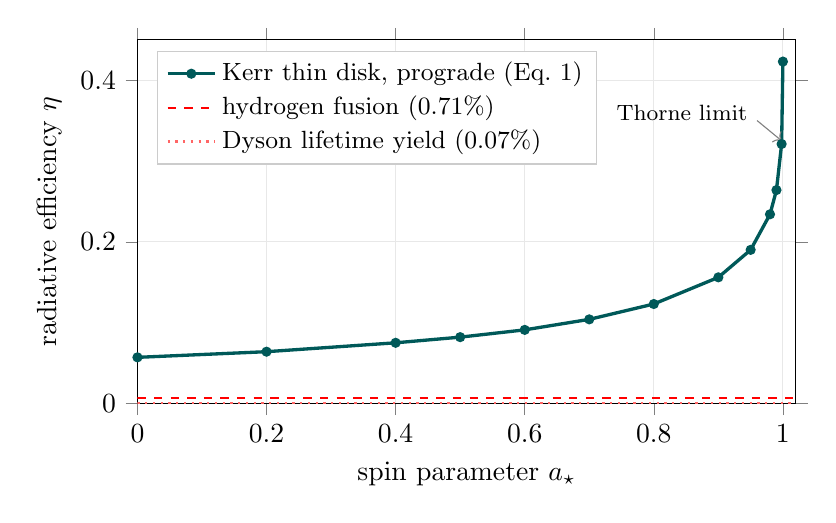
\begin{tikzpicture}
\begin{axis}[width=0.82\textwidth,height=6.2cm,
  xlabel={spin parameter $\astar$}, ylabel={radiative efficiency $\eta$},
  xmin=0,xmax=1.02,ymin=0,ymax=0.45,
  grid=both,grid style={gray!18},tick align=outside,
  legend pos=north west,legend cell align=left,legend style={font=\small,draw=gray!40}]
\addplot[teal!70!black,very thick,mark=*,mark size=1.2pt] coordinates {
 (0,0.057)(0.2,0.064)(0.4,0.075)(0.5,0.082)(0.6,0.091)(0.7,0.104)
 (0.8,0.123)(0.9,0.156)(0.95,0.190)(0.98,0.234)(0.99,0.264)(0.998,0.321)(1,0.423)};
\addlegendentry{Kerr thin disk, prograde (Eq.~1)}
\addplot[red,dashed,thick,domain=0:1.02,samples=2]{0.0071};
\addlegendentry{hydrogen fusion ($0.71\%$)}
\addplot[red!60,dotted,thick,domain=0:1.02,samples=2]{0.0007};
\addlegendentry{Dyson lifetime yield ($0.07\%$)}
\node[font=\footnotesize,anchor=east] at (axis cs:0.96,0.36) {Thorne limit};
\draw[gray,->] (axis cs:0.96,0.35)--(axis cs:0.998,0.325);
\end{axis}
\end{tikzpicture}
\caption{Mass-to-energy conversion efficiency of thin-disk accretion as a function of black-hole spin \citep{bardeen1972,novikov1973}, compared with hydrogen fusion and with the lifetime yield of Dyson-type stellar harvesting. The \citet{thorne1974} limit $\astar = 0.998$ ($\eta \approx 0.32$) marks the equilibrium spin reachable by disk accretion alone. Curve drawn through values of Eq.~(1) at the plotted points.}
\label{fig:eff}
\end{figure}

\paragraph{Power throughput.} The sustainable luminosity is bounded by the Eddington limit,
\begin{equation}
L_{\rm Edd} = \frac{4\pi G M m_p c}{\sigma_T} \approx 1.26\times10^{31}\,(M/\msun)\ \mathrm{W},
\end{equation}
giving $1.0\times10^{35}$, $2.5\times10^{35}$, and $6.3\times10^{35}$~W at $M = 8.2\times10^{3}$, $2\times10^{4}$, and $5\times10^{4}\,\msun$ respectively \citep{frank2002,shapiro1983}---some ${\sim}10^{9}$ times the bolometric output of the Sun, and hence of any solar Dyson swarm (Fig.~\ref{fig:power}). The corresponding Eddington accretion rate, $\dot{M}_{\rm Edd} = L_{\rm Edd}/\eta c^{2}$, is remarkably modest: at $\eta = 0.1$ and $M = 2\times10^{4}\,\msun$, one solar mass sustains the limit for ${\sim}2{,}300$~years. A globular-cluster core containing $\gtrsim 10^{5}$ stars within its central parsec can therefore fuel Eddington-limited operation for ${\sim}10^{8\text{--}9}$~years using bodies that no fusion-based economy values.

\begin{figure}[t]
\centering
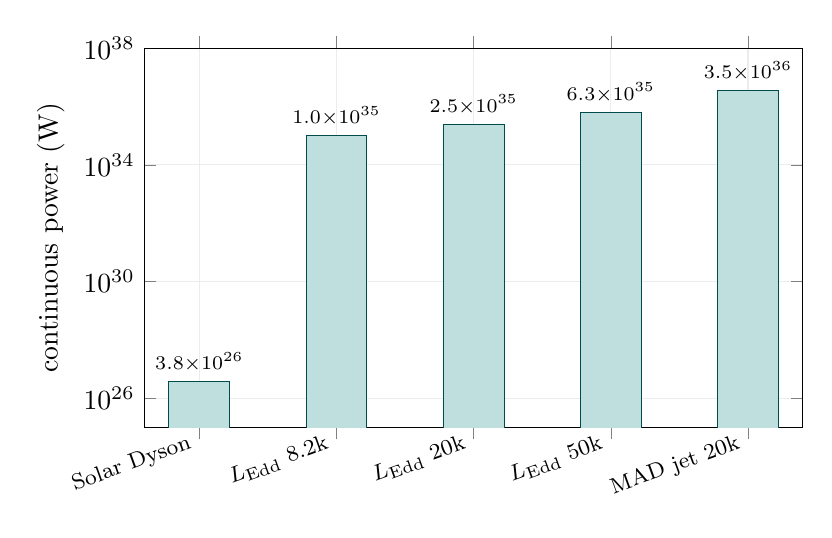
\begin{tikzpicture}
\begin{axis}[width=0.82\textwidth,height=6.4cm,
  ybar,bar width=22pt,ymode=log,
  ymin=1e25,ymax=1e38,ylabel={continuous power (W)},
  symbolic x coords={dyson,edd8,edd20,edd50,mad},
  xtick=data,
  xticklabels={Solar Dyson,$L_{\rm Edd}$ 8.2k,$L_{\rm Edd}$ 20k,$L_{\rm Edd}$ 50k,MAD jet 20k},
  x tick label style={font=\footnotesize,rotate=20,anchor=east},
  grid=both,grid style={gray!15}]
\addplot[draw=teal!60!black,fill=teal!25] coordinates {
 (dyson,3.8e26)(edd8,1.0e35)(edd20,2.5e35)(edd50,6.3e35)(mad,3.5e36)};
\node[font=\scriptsize,anchor=south] at (axis cs:dyson,3.8e26){$3.8{\times}10^{26}$};
\node[font=\scriptsize,anchor=south] at (axis cs:edd8,1.0e35){$1.0{\times}10^{35}$};
\node[font=\scriptsize,anchor=south] at (axis cs:edd20,2.5e35){$2.5{\times}10^{35}$};
\node[font=\scriptsize,anchor=south] at (axis cs:edd50,6.3e35){$6.3{\times}10^{35}$};
\node[font=\scriptsize,anchor=south] at (axis cs:mad,3.5e36){$3.5{\times}10^{36}$};
\end{axis}
\end{tikzpicture}
\caption{Continuous power available from a complete solar Dyson swarm versus Eddington-limited accretion (Eq.~2) onto IMBHs spanning the contested $\acen$ mass range, and a magnetically arrested (MAD) Blandford--Znajek jet at $\astar \approx 0.99$ with $\eta_{\rm jet} \approx 1.4$ \citep{tchekhovskoy2011}, fed at the $\eta = 0.1$ Eddington rate. The IMBH advantage in instantaneous power is roughly nine orders of magnitude.}
\label{fig:power}
\end{figure}

\paragraph{Spin energy and the Blandford--Znajek channel.} A Kerr hole stores extractable rotational energy
\begin{equation}
E_{\rm rot} = \left[1 - \sqrt{\tfrac{1}{2}\left(1 + \sqrt{1 - \astar^{2}}\right)}\,\right] M c^{2},
\end{equation}
reaching $0.29\,Mc^{2} \approx 1.0\times10^{51}$~J for $M = 2\times10^{4}\,\msun$ as $\astar \to 1$---a reservoir equal to the entire lifetime fusion output of ${\sim}10^{7}$ Suns, storable indefinitely and tappable on demand. That this energy is extractable in principle was shown by the ergosphere mechanism of \citet{penrose1969} and \citet{penrose1971}; the astrophysically efficient extraction mechanism is electromagnetic: a horizon threaded by poloidal magnetic flux $\Phi$ acts as a unipolar inductor, driving Poynting-flux jets with power $P_{\rm BZ} \propto \Phi^{2}\Omega_H^{2}$ \citep{blandford1977}. In the magnetically arrested disk (MAD) regime, general-relativistic magnetohydrodynamic simulations find jet efficiencies $\eta_{\rm jet} \equiv P_{\rm jet}/\dot{M}c^{2} \approx 1.4$ at $\astar \approx 0.99$ \citep{tchekhovskoy2011,tchekhovskoy2015}---the jet carries \emph{more} energy than the accreted rest mass, the excess drawn from spin. The BZ scaling has recently been confirmed from first principles by ab-initio particle-in-cell simulations of Kerr magnetospheres \citep{meringolo2025}, which additionally identify equatorial magnetic reconnection as a supplementary extraction channel \citep{comisso2021,camilloni2025}; one 2026 preprint reports transient MAD states with jet power exceeding accretion power by over two orders of magnitude \citep[][not yet peer-reviewed]{nathanail2026}. For the MTH it suffices that $\eta_{\rm jet} \gtrsim 1$ is robust across methods.

\paragraph{Spin-up economics.} A hole of low natal spin is itself improvable. Prograde thin-disk accretion drives $\astar \to 0.998$ after the hole grows by a factor ${\approx}2.4$ \citep{thorne1974}; for an initial $2\times10^{4}\,\msun$ hole this costs ${\sim}3\times10^{4}\,\msun$ of accreted matter and, at Eddington throughput, ${\sim}10^{8}$~years. The investment multiplies all subsequent per-unit-fuel returns by up to ${\sim}6$ (Fig.~\ref{fig:eff}) and unlocks the BZ reservoir. We emphasize the corollary for observers: \emph{spin is the single most diagnostic parameter of the system's history} (Section~\ref{sec:falsification}), since natural IMBH formation channels do not generically predict near-extremal spin, whereas the MTH requires engineered systems to approach it.

\subsection{Entropy disposal: the horizon as the ultimate cold reservoir}\label{sec:landauer}
Landauer's principle sets the minimum thermodynamic cost of irreversible computation: erasing one bit dissipates at least $k_B T \ln 2$ into a reservoir at temperature $T$ \citep{landauer1961,bennett1982,parrondo2015}, a bound verified experimentally \citep{berut2012}. Reversible logic evades the bound for intermediate steps \citep{bennett1973,toffoli1980,fredkin1982,athas1994,frank2002b}, but error correction, measurement, and memory reuse impose a residual erasure budget on any real computer \citep{wolpert2019}. For a conventional deep-space computer the reservoir floor is the CMB at $T_\gamma = 2.7$~K, so the marginal cost is $k_B T_\gamma \ln 2 = 2.6\times10^{-23}$~J per bit. This is the floor that aestivation proposes to lower by waiting ${\sim}10^{12}$~years \citep{sandberg2016}.

An event horizon lowers it \emph{now}. By the generalized second law, the sum of black-hole entropy $S_{\rm BH} = k_B c^{3} A/4G\hbar$ and exterior entropy is non-decreasing, and entropy carried across the horizon is accounted by the area increase \citep{bekenstein1973,bekenstein1974,bousso2002}. The marginal energy cost of horizon disposal is set by the horizon temperature
\begin{equation}
T_H = \frac{\hbar c^{3}}{8\pi G M k_B} \approx 6.2\times10^{-8}\,(\msun/M)\ \mathrm{K}
\end{equation}
\citep{hawking1974,hawking1975}: $T_H \approx 3\times10^{-12}$~K at $2\times10^{4}\,\msun$---\emph{twelve orders of magnitude below the CMB}. A bit dumped at the horizon costs $k_B T_H \ln 2 \sim 3\times10^{-35}$~J against $2.6\times10^{-23}$~J for CMB radiation (Fig.~\ref{fig:landauer}). This single substitution captures essentially the entire ${\sim}10^{30}$ efficiency factor that motivated aestivation---without waiting, and therefore without forfeiting the free energy that \citet{bennett2019} showed dormant civilizations irretrievably lose.

\begin{figure}[t]
\centering
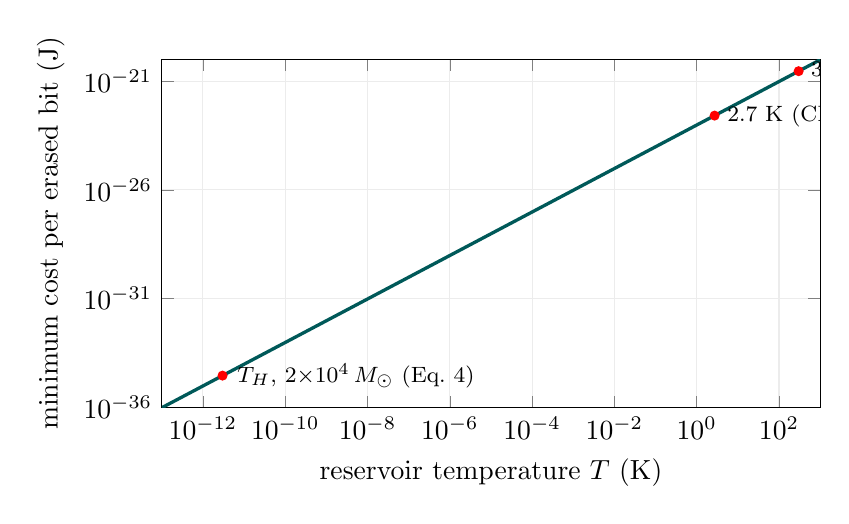
\begin{tikzpicture}
\begin{axis}[width=0.82\textwidth,height=6cm,
  xmode=log,ymode=log,
  xlabel={reservoir temperature $T$ (K)}, ylabel={minimum cost per erased bit (J)},
  xmin=1e-13,xmax=1e3,ymin=1e-36,ymax=1e-20,
  grid=both,grid style={gray!15}]
\addplot[teal!70!black,very thick,domain=1e-13:1e3,samples=2]{9.57e-24*x};
\addplot[red,only marks,mark=*,mark size=1.6pt] coordinates {(300,2.87e-21)(2.725,2.6e-23)(3e-12,2.87e-35)};
\node[font=\footnotesize,anchor=west] at (axis cs:350,2.87e-21){300 K (terrestrial)};
\node[font=\footnotesize,anchor=west] at (axis cs:3.2,2.6e-23){2.7 K (CMB floor)};
\node[font=\footnotesize,anchor=west] at (axis cs:4e-12,2.87e-35){$T_H$, $2{\times}10^{4}\,M_\odot$ (Eq.~4)};
\end{axis}
\end{tikzpicture}
\caption{Landauer cost per erased bit, $k_B T \ln 2$, as a function of reservoir temperature. Dumping waste entropy across an IMBH horizon (marginal temperature $T_H$, Eq.~4) rather than radiating to the CMB lowers the erasure floor by ${\sim}10^{12}$, in the present epoch, consistent with the generalized second law \citep{bekenstein1974}.}
\label{fig:landauer}
\end{figure}

\subsection{Information storage: the Bekenstein--Hawking archive}
The Bekenstein bound limits the information content of any bounded system \citep{bekenstein1981,casini2008}; black holes saturate it, with
\begin{equation}
S_{\rm BH}/(k_B \ln 2) \approx 1.5\times10^{77}\,(M/\msun)^{2}\ \text{bits},
\end{equation}
i.e.\ ${\sim}6\times10^{85}$ bits at $2\times10^{4}\,\msun$ \citep{bekenstein1973,lloyd2000}. Information crossing the horizon is scrambled but, by unitarity, not destroyed; retrieval timescales via Hawking radiation are, however, of order the evaporation time, ${\sim}10^{67}(M/\msun)^{3}$~yr \citep{page1976}---the archive is functionally write-only. Black holes likewise saturate the Margolus--Levitin bound on processing rate, $2E/\pi\hbar$ operations per second \citep{margolus1998,lloyd2000}.

\subsection{Time dilation as an engineering parameter}
A platform on a circular equatorial geodesic at radius $r$ around a Kerr hole runs slow relative to infinity by
\begin{equation}
\frac{d\tau}{dt} = \frac{\sqrt{1 - 3 r_g/r + 2\astar (r_g/r)^{3/2}}}{1 + \astar (r_g/r)^{3/2}}
\end{equation}
\citep{bardeen1972}: $d\tau/dt = \sqrt{1/2} \approx 0.707$ at the Schwarzschild ISCO, falling to ${\approx}0.093$ (a factor ${\sim}11$) at the prograde ISCO for $\astar = 0.998$ (Fig.~\ref{fig:isco}). Larger factors require powered non-geodesic hovering at diverging thrust cost; popular claims of $1000{:}1$ dilation at stable orbits are incorrect by 1--2 orders of magnitude. A tiered swarm can therefore place archival processes deep and interactive processes high, with the choice of orbit acting as a clock-rate dial.

\begin{figure}[t]
\centering
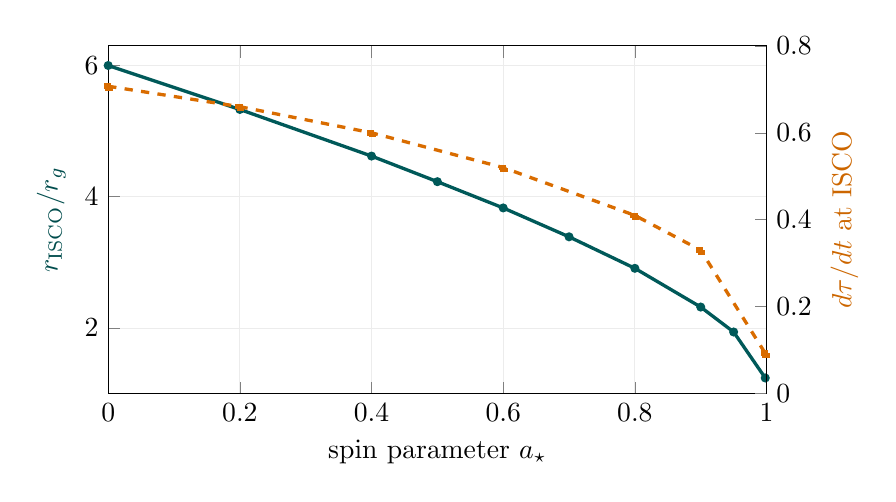
\begin{tikzpicture}
\begin{axis}[width=0.82\textwidth,height=6cm,
  axis y line*=left,xmin=0,xmax=1,ymin=1,ymax=6.3,
  xlabel={spin parameter $\astar$}, ylabel={$r_{\rm ISCO}/r_g$},
  y label style={text=teal!60!black},
  grid=major,grid style={gray!15}]
\addplot[teal!70!black,very thick,mark=*,mark size=1pt] coordinates {
 (0,6)(0.2,5.33)(0.4,4.62)(0.5,4.23)(0.6,3.83)(0.7,3.39)(0.8,2.91)(0.9,2.32)(0.95,1.94)(0.998,1.24)};
\label{plt:risco}
\end{axis}
\begin{axis}[width=0.82\textwidth,height=6cm,
  axis y line*=right,axis x line=none,xmin=0,xmax=1,ymin=0,ymax=0.8,
  ylabel={$d\tau/dt$ at ISCO},
  y label style={text=orange!80!black}]
\addplot[orange!85!black,very thick,dashed,mark=square*,mark size=1pt] coordinates {
 (0,0.707)(0.2,0.66)(0.4,0.60)(0.6,0.52)(0.8,0.41)(0.9,0.33)(0.998,0.093)};
\end{axis}
\end{tikzpicture}
\caption{Prograde ISCO radius (left axis, teal) and proper-time ratio for a circular geodesic at the ISCO (right axis, orange) as functions of spin \citep{bardeen1972}. Spin-up from $\astar = 0$ to the Thorne limit moves the working orbit from $6\,r_g$ to ${\sim}1.24\,r_g$ and deepens the available stable time dilation from $1.41{:}1$ to ${\sim}11{:}1$.}
\label{fig:isco}
\end{figure}

\subsection{Why inward beats outward for a computation-maximizer}
The expansionist default implicitly maximizes \emph{resource acquisition}; P1 civilizations maximize \emph{computation}, and the two diverge. Expansion multiplies harvested mass at most polynomially in time while imposing light-lag decoherence on any shared computation. Concentration multiplies the \emph{yield per unit mass} by the factors of Section~\ref{sec:thermo} (up to ${\sim}600$ over Dyson harvesting), lowers the erasure floor by ${\sim}10^{12}$ (Section~\ref{sec:landauer}), and keeps the entire system within light-seconds of itself. For any utility function dominated by total integrated computation, the gradient points inward once beamed-sail transport makes a cluster-hosted IMBH reachable at negligible marginal cost \citep{lubin2016,armstrong2013}. P1 requires only that \emph{some} civilizations follow this gradient.

\section{Omega Centauri as the optimal observational target}\label{sec:omegacen}
\subsection{The cluster}
$\acen$ is the most massive Galactic globular cluster ($M_{\rm cl} \approx 4\times10^{6}\,\msun$, ${\sim}10^{7}$ stars; \citealp{baumgardt2018}), at a kinematic distance of $5.49 \pm 0.06$~kpc \citep{haberle2025}, consistent within systematics with the Gaia EDR3 parallax ($5.24 \pm 0.11$~kpc; \citealp{soltis2021}) and the combined catalogue value ($5.43 \pm 0.05$~kpc; \citealp{baumgardt2021}). It hosts multiple stellar populations spanning a broad metallicity range \citep{johnson2010}, a mean stellar age of $12.08 \pm 0.01$~Gyr with an intrinsic spread of $0.75$~Gyr \citep{clontz2024}, significant rotation, and an associated tidal stream \citep{ibata2019}---the consensus interpretation being that it is the surviving nucleus of a dwarf galaxy accreted and stripped by the Milky Way \citep{hilker2000,bekki2019}. Table~\ref{tab:params} summarizes the adopted parameters. For the selection criteria of Section~\ref{sec:selection}, the stripped-nucleus origin matters twice over: nuclear star clusters are the environments most likely to form and retain IMBHs \citep{greene2020}, and the age structure implies that any technological lineage has had $\gtrsim 8$~Gyr to locate, reach, and develop the system.

\begin{table}[t]
\centering
\caption{Adopted parameters for $\acen$ (NGC~5139).}
\label{tab:params}
\small
\begin{tabular}{@{}lll@{}}
\toprule
Quantity & Value & Source \\
\midrule
Distance & $5.49 \pm 0.06$~kpc & \citet{haberle2025} \\
Cluster mass & ${\approx}\,4\times10^{6}\,\msun$ & \citet{baumgardt2018} \\
Stellar count & ${\sim}10^{7}$ & \citet{baumgardt2018} \\
Mean stellar age & $12.08 \pm 0.01$~Gyr (spread $0.75$~Gyr) & \citet{clontz2024} \\
Origin & stripped dwarf-galaxy nucleus & \citet{hilker2000,ibata2019} \\
Central density & ${\sim}10^{3}\,\msun\,\mathrm{pc}^{-3}$ & \citet{pryor1993} \\
Declination & $-47.5^{\circ}$ & \citet{harris1996} \\
\bottomrule
\end{tabular}
\end{table}

\subsection{The IMBH candidate and the mass tension}
Evidence for a central dark mass in $\acen$ has accumulated for two decades, from integrated kinematics \citep{noyola2008} through proper-motion modelling that initially yielded only upper limits at the ${\sim}10^{4}\,\msun$ level \citep{vandermarel2010}, with stellar-mass black-hole subsystems long advanced as the alternative \citep{zocchi2019,breen2013}. The situation changed when \citet{haberle2024a}, using a proper-motion catalogue of 1.4~million stars built from over 500 HST epochs \citep{haberle2024b}, identified seven stars within 3~arcsec of the cluster centre moving faster than the local escape velocity. Their velocities alone require a point mass $\ge 8{,}200\,\msun$; including acceleration limits raises the lower bound to $21{,}100\,\msun$ at 99 per cent confidence. Independent $N$-body modelling finds that an IMBH grown in situ to ${\sim}5\times10^{4}\,\msun$ reproduces the present-day cluster structure and fast-star population \citep{gonzalez2025}.

Against this stands \citet{banares2025}: a joint analysis of stellar kinematics and timing accelerations of the cluster's millisecond pulsars that places a $3\sigma$ \emph{upper} limit of ${\sim}6\times10^{3}\,\msun$ on any central point mass, favouring instead an \emph{extended} central dark component of ${\approx}2$--$3\times10^{5}\,\msun$. The two results are formally inconsistent under each side's stated modelling assumptions (Table~\ref{tab:masstension}). We take no side; the MTH requires a genuine IMBH (P2), so the Bañares-Hernández scenario, if confirmed, falsifies the $\acen$ application outright. LISA will settle the question: a single IMBH yields resolvable extreme-mass-ratio-inspiral (EMRI) signals with percent-level mass and spin measurement, whereas a remnant swarm yields a qualitatively different signature \citep{amaroseoane2018,babak2017,colpi2024}.

\begin{table}[t]
\centering
\caption{Current constraints on the central dark mass of $\acen$. The kinematic lower bounds and the pulsar-timing upper bound are mutually inconsistent under stated assumptions.}
\label{tab:masstension}
\small
\begin{tabular}{@{}lll@{}}
\toprule
Constraint & Value & Method / source \\
\midrule
Lower bound (velocities only) & $\ge 8{,}200\,\msun$ & 7 fast stars, HST PMs \citep{haberle2024a} \\
Lower bound (with accelerations) & $\ge 21{,}100\,\msun$ (99\%) & same stars, accel.\ limits \citep{haberle2024a} \\
$N$-body growth models & ${\sim}4.7$--$5.1\times10^{4}\,\msun$ & cluster evolution \citep{gonzalez2025} \\
Upper bound (point mass) & $< 6\times10^{3}\,\msun$ ($3\sigma$) & kinematics + MSP timing \citep{banares2025} \\
Favoured alternative & extended $2$--$3\times10^{5}\,\msun$ & same analysis \citep{banares2025} \\
Historical upper limits & $\lesssim 10^{4}\,\msun$ (model-dep.) & HST PMs \citep{vandermarel2010,zocchi2019} \\
\bottomrule
\end{tabular}
\end{table}

\subsection{Electromagnetic silence}
Whatever occupies the centre of $\acen$, it is extraordinarily dark. The deepest radio observation of any globular cluster---${\sim}170$~h with ATCA at $7.25$~GHz, reaching an rms of $1.1\,\mu$Jy\,beam$^{-1}$---detects nothing at any proposed cluster centre, bounding the accretion efficiency of a putative IMBH at $\varepsilon \lesssim 4\times10^{-3}$ of the Bondi rate ($3\sigma$) \citep{mahida2026}. JWST NIRCam and MIRI photometry likewise finds no source with the spectral energy distribution of an accreting IMBH \citep{chen2025}. No dedicated technosignature search of $\acen$ has ever been conducted at any wavelength; the first dedicated globular-cluster SETI survey \citep{huang2026} could not observe $\acen$ from FAST's latitude. We are emphatic about the logic: electromagnetic silence is \emph{predicted} by the MTH (P3--P4), but it is equally consistent with---and more parsimoniously explained by---a quiescent, gas-starved compact object, which we adopt as the null hypothesis $H_0$ throughout.

\subsection{Why not Sagittarius A*?}\label{sec:sgra}
A natural objection: if bigger is better, the Galactic Centre hosts a $4.3\times10^{6}\,\msun$ hole \citep{gravity2022,eht2022} with abundant fuel. Three of the four selection criteria disfavour it. First, the storage and erasure advantages saturate at IMBH scale. Second, the Galactic Centre is the most dynamically violent environment in the Galaxy---the opposite of a stable substrate for Gyr-scale infrastructure; $\acen$'s relaxed core offers the same physics with none of the weather. Third, the Galactic Centre's gas and stars are the future fuel of natural astrophysics and conceivably of competitors, whereas a globular cluster's low-mass stellar reservoir is valueless to any fusion-era civilization.

\section{A staged exploitation architecture}\label{sec:architecture}
\epistemic{\textbf{Epistemic status:} This section is speculative civilizational engineering. It is included not as prediction but because the falsification program of Section~\ref{sec:falsification} requires a concrete model of \emph{what would be observable at each stage}.}

We model the migration as five phases (Fig.~\ref{fig:phases}), parameterized for a civilization departing a planetary system ${\sim}5$~kpc from $\acen$.

\begin{description}[leftmargin=0pt]
\item[Phase 1 --- Scouts.] Gram-scale beamed-sail probes at $0.1$--$0.2c$ \citep{lubin2016}; transit ${\sim}10^{5}$~yr. \emph{External signature: none detectable at interstellar range.}
\item[Phase 2 --- Self-replicating industry.] Kilogram-scale seed factories bootstrap from asteroidal material \citep{freitas1982}. \emph{Signature: waste heat far below detectability.}
\item[Phase 3 --- ISCO computronium swarm.] The main payload assembles a free-flying compute swarm near the ISCO; BZ extraction begins at low spin. \emph{Signature: faint soft accretion luminosity---the one conventionally observable phase; current limits \citep{mahida2026,chen2025} already exclude an active Phase~3 above ${\sim}10^{-3}$ Eddington.}
\item[Phase 4 --- Spin-up.] Sustained prograde feeding (${\sim}10^{4\text{--}5}$ stars over ${\sim}10^{8}$~yr) drives $\astar \to 0.9$--$0.998$. \emph{Signature: secular cluster-core depletion; episodic jet activity; high spin as a permanent record.} Phases~3--5 presuppose institutional or goal stability over $10^{8}$~yr---the architecture's largest unargued premise.
\item[Phase 5 --- Endpoint.] Near-extremal spin; waste entropy disposed across the horizon; the system is thermodynamically silent. The sole conjectured emission channel is burst-mode high-energy neutrinos if manufactured micro black holes are employed per \citet{dvali2023}; their formation may be blocked by Schwinger-limit pair production \citep{alvarez2024,breit1934,schwinger1951}, a conclusion contested by \citet{loeb2024}.
\end{description}

\begin{figure}[t]
\centering
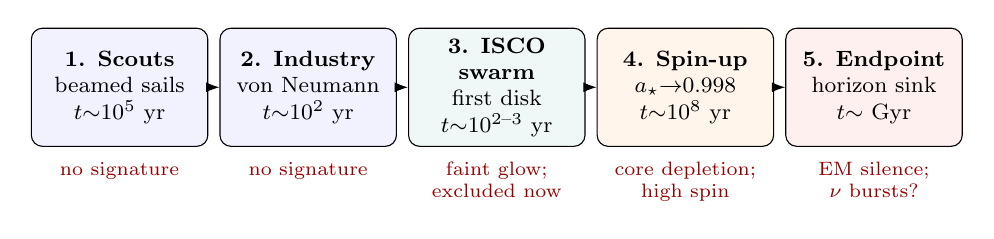
\begin{tikzpicture}[font=\footnotesize,node distance=4pt,
  pbox/.style={draw,rounded corners,align=center,text width=2.1cm,minimum height=1.5cm,inner sep=2pt},
  sig/.style={align=center,text width=2.1cm,font=\scriptsize,red!60!black}]
\node[pbox,fill=blue!5] (p1) {\textbf{1. Scouts}\\beamed sails\\$t{\sim}10^5$ yr};
\node[pbox,fill=blue!5,right=of p1] (p2) {\textbf{2. Industry}\\von Neumann\\$t{\sim}10^2$ yr};
\node[pbox,fill=teal!6,right=of p2] (p3) {\textbf{3. ISCO swarm}\\first disk\\$t{\sim}10^{2\text{--}3}$ yr};
\node[pbox,fill=orange!8,right=of p3] (p4) {\textbf{4. Spin-up}\\$\astar{\to}0.998$\\$t{\sim}10^8$ yr};
\node[pbox,fill=red!6,right=of p4] (p5) {\textbf{5. Endpoint}\\horizon sink\\$t{\sim}$ Gyr};
\draw[-{Latex}] (p1)--(p2); \draw[-{Latex}] (p2)--(p3);
\draw[-{Latex}] (p3)--(p4); \draw[-{Latex}] (p4)--(p5);
\node[sig,below=2pt of p1]{no signature};
\node[sig,below=2pt of p2]{no signature};
\node[sig,below=2pt of p3]{faint glow; excluded now};
\node[sig,below=2pt of p4]{core depletion; high spin};
\node[sig,below=2pt of p5]{EM silence; $\nu$ bursts?};
\end{tikzpicture}
\caption{The five-phase exploitation architecture (speculative) and the external signature of each phase (red). Only Phase~3 is conventionally luminous; the permanent observables are dynamical (spin, core depletion), which is why gravitational-wave spin measurement is the decisive test.}
\label{fig:phases}
\end{figure}

\section{Falsification framework and observational program}\label{sec:falsification}
A hypothesis earns scientific standing by what it risks. We define three competing hypotheses: $H_0$ (gas starvation; null)---the central object is silent for the ordinary reason; $H_1$ (dark remnant swarm)---no IMBH exists \citep{banares2025,zocchi2019,breen2013}, which falsifies the $\acen$ application; and $H_2$ (MTH)---an IMBH exists and is, or has been, the substrate of a migrated civilization. $H_0$ and $H_2$ predict identical electromagnetic appearances today, so electromagnetic non-detections cannot distinguish them; they diverge on dynamical and high-energy observables. Table~\ref{tab:falsification} states six tests with thresholds, instruments, and timelines; Fig.~\ref{fig:tree} arranges the decisive subset as a decision tree.

\begin{table}[t]
\centering
\caption{Falsification matrix for the MTH at $\acen$. Tests marked $\dagger$ are decisive against the hypothesis as a whole. LISA timeline assumes launch in the mid-2030s \citep{colpi2024}.}
\label{tab:falsification}
\footnotesize
\begin{tabular}{@{}p{0.5cm}p{3.5cm}p{3.6cm}p{2.2cm}p{2.4cm}@{}}
\toprule
\# & Observation & Threshold & Instrument & Kills \\
\midrule
T1 & Accretion luminosity from core & $L_{\rm acc} > 10^{29}$~W sustained ${>}1$~yr & JWST MIRI; ATCA/MeerKAT; Chandra & Phase 5 mgmt.; already constrained \\
T2 & Mid-IR waste-heat excess & ${>}3\sigma$ over stellar model, 10--30\,$\mu$m & JWST MIRI & any Dyson capture; Phases 4--5 \\
T3$\dagger$ & GW signature inconsistent with single point mass & stochastic bkg.\ or multiple low-mass inspirals & LISA & $H_2$ entirely (confirms $H_1$) \\
T4$\dagger$ & EMRI point mass too small & clean chirp, $M < 5\times10^{3}\,\msun$ at ${>}3\sigma$ & LISA & $H_2$ at $\acen$ \\
T5$\dagger$ & EMRI spin measurement low & $\astar < 0.1$ at ${>}3\sigma$ & LISA & the exploitation model \\
T6 & High-energy neutrino bursts & $\ge 3$ tracks within $1^{\circ}$ in $10^{2\text{--}3}$~s, $E \gtrsim 10$~TeV & KM3NeT/ARCA & closes Dvali--Osmanov channel \\
\bottomrule
\end{tabular}
\end{table}

The single most informative number obtainable this generation is the \emph{LISA spin measurement}: $H_0$ makes no strong spin prediction, while a measured $\astar \gtrsim 0.9$ on a gas-starved IMBH that has accreted nothing for Gyr would be difficult to explain naturally and is the MTH's flagship residue (P4a). EMRI parameter estimation at LISA delivers spin to better than percent precision for favourable systems \citep{babak2017,amaroseoane2018}. The program is cheap: T1--T2 are archival or piggyback analyses; T6 requires only a pointed monitoring program on an instrument already built for the southern sky \citep{adrian2016,km3net2025}, following the high-energy SETI logic of \citet{lacki2025} and standard point-source pipelines \citep{icecube2020}; and T3--T5 are free by-products of LISA's planned EMRI science \citep{colpi2024}.

\begin{figure}[t]
\centering
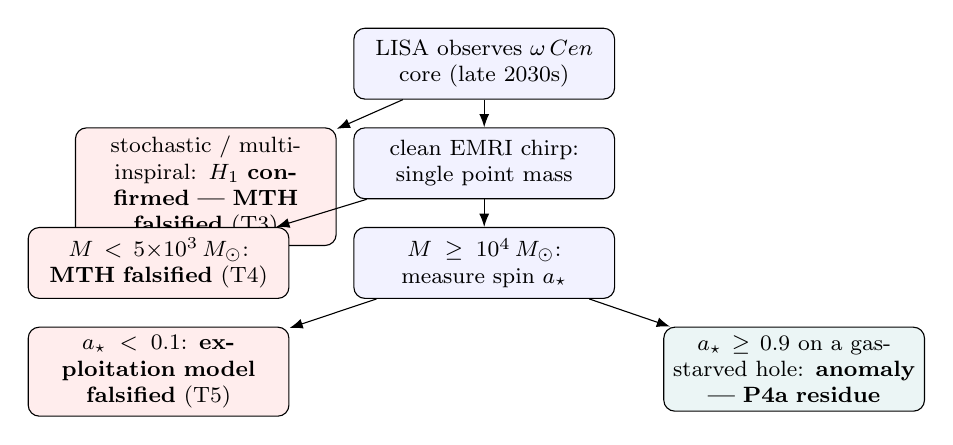
\begin{tikzpicture}[font=\footnotesize,node distance=10pt and 6pt,
  nd/.style={draw,rounded corners,align=center,text width=3.1cm,inner sep=3pt,minimum height=0.9cm},
  kill/.style={nd,fill=red!7},live/.style={nd,fill=teal!8},mid/.style={nd,fill=blue!5}]
\node[mid] (root) {LISA observes $\acen$ core (late 2030s)};
\node[kill,below left=of root] (swarm) {stochastic / multi-inspiral: \textbf{$H_1$ confirmed --- MTH falsified} (T3)};
\node[mid,below=of root] (emri) {clean EMRI chirp: single point mass};
\node[kill,below left=of emri,xshift=-0.6cm] (small) {$M<5{\times}10^{3}\,\msun$: \textbf{MTH falsified} (T4)};
\node[mid,below=of emri] (large) {$M\ge 10^{4}\,\msun$: measure spin $\astar$};
\node[kill,below left=of large,xshift=-0.6cm] (lospin) {$\astar<0.1$: \textbf{exploitation model falsified} (T5)};
\node[live,below right=of large,xshift=0.4cm] (hispin) {$\astar\ge0.9$ on a gas-starved hole: \textbf{anomaly --- P4a residue}};
\draw[-{Latex}] (root)-- (swarm); \draw[-{Latex}] (root)--(emri);
\draw[-{Latex}] (emri)--(small); \draw[-{Latex}] (emri)--(large);
\draw[-{Latex}] (large)--(lospin); \draw[-{Latex}] (large)--(hispin);
\end{tikzpicture}
\caption{Decision tree for the decisive (gravitational-wave) branch of the falsification program. Red boxes terminate the hypothesis or its exploitation model; the single shaded branch is the only outcome in which the MTH gains material support, and even there the inference is to ``anomaly requiring explanation,'' not detection.}
\label{fig:tree}
\end{figure}

\paragraph{What would count as support.} The MTH gains support only from conjunctions that $H_0$ finds awkward: (i)~a LISA-confirmed IMBH with $\astar \gtrsim 0.9$ \emph{despite} Gyr-scale gas starvation; (ii)~repeated ${>}5\sigma$ neutrino bursts from the core with hard spectra and no electromagnetic counterpart; or (iii)~astrometric evidence of statistically anomalous depletion of loosely bound core stars. No single line would constitute proof of technology. Conversely, we commit in advance: if LISA delivers T3, T4, or T5, the $\acen$ application of the MTH should be retired without special pleading.

\section{Discussion: objections and limits}\label{sec:discussion}
\paragraph{Parsimony.} The MTH posits extraterrestrial intelligence; $H_0$ posits nothing. By any reasonable prior the null is favoured, and we have structured every comparison accordingly. The defensible claim is not that the MTH is probable but that it is \emph{cheap to test relative to its information value}.

\paragraph{The anthropic objection.} The MTH explains the silence of the old, not the existence of the young; it thins the expected population of loud civilizations by removing its most capable members, sharpening rather than fully dissolving the paradox \citep{hanson2021}.

\paragraph{Goal stability over $10^{8}$ years.} Phase~4 presupposes coherent purpose across timescales that dwarf all institutional experience---the architecture's largest unargued premise. One partial mitigation: the payoff structure is front-loaded, so a lineage that fragments mid-program still leaves the P4 dynamical residues that our tests target.

\paragraph{Tidal and radiative survivability at the ISCO.} At $2\times10^{4}\,\msun$ the tidal field at the Schwarzschild ISCO is $2GM/r_{\rm ISCO}^{3} \approx 1$~s$^{-2}$: a 10-m node experiences a benign ${\sim}1g$ differential, motivating a swarm of small free-flying nodes rather than a monolithic platform.

\paragraph{Scope of the $\acen$ bet.} The MTH is a selection theory over a class; $\acen$ is its highest-ranked accessible member, not its definition. We bind ourselves to the class-level prediction: \emph{if no Galactic globular-cluster IMBH with $\astar \gtrsim 0.9$ exists, the MTH is wrong for the Milky Way}, a statement LISA-era gravitational-wave astronomy can settle.

\section{Conclusion}\label{sec:conclusion}
We have argued, first as a matter of established physics, that rapidly spinning massive black holes in dense old stellar clusters constitute the global optimum among present-day environments for long-term computation---by factors of ${\sim}10^{2}$ in energy per unit fuel, ${\sim}10^{9}$ in continuous power, ${\sim}10^{12}$ in entropy-disposal cost, and unbounded factors in archival density---and second, as an explicitly speculative hypothesis, that this gradient acts on the oldest technological civilizations as an attractor whose operation would look, from outside, exactly like the silence we observe. The Macro Transcension Hypothesis inherits the thermodynamic insight of transcension and aestivation while repairing their respective defects: it needs no exit from the universe and no dormancy, and it survives the Bennett--Hanson--Riedel free-energy objection by importing the cold reservoir into the present. Its principal virtue is that it pays its way observationally---selecting a named target whose contested central object, perfect electromagnetic silence, and 12-Gyr head start make it scientifically urgent on entirely conventional grounds, and committing to kill criteria that existing and funded instruments will adjudicate.

\section*{Acknowledgements and disclosure}
\textbf{AI assistance disclosure:} drafting, citation verification, derivation checking, and figure preparation were performed with substantial assistance from a large language model (Claude, Anthropic), under the author's direction; the author reviewed and takes full responsibility for all claims, derivations, and references.

\begin{thebibliography}{99}
\small
\bibitem[Adri\'an-Mart\'inez et al.(2016)]{adrian2016} Adri\'an-Mart\'inez, S., et al.\ (KM3NeT Collaboration) (2016). Letter of intent for KM3NeT 2.0. \emph{J.\ Phys.\ G}, 43, 084001.
\bibitem[\'Alvarez-Dom\'inguez et al.(2024)]{alvarez2024} \'Alvarez-Dom\'inguez, \'A., Garay, L.~J., Mart\'in-Mart\'inez, E., \& Polo-G\'omez, J. (2024). No black holes from light. \emph{Phys.\ Rev.\ Lett.}, 133, 041401.
\bibitem[Amaro-Seoane(2018)]{amaroseoane2018} Amaro-Seoane, P. (2018). Relativistic dynamics and extreme mass ratio inspirals. \emph{Living Rev.\ Relativ.}, 21, 4.
\bibitem[Armstrong \& Sandberg(2013)]{armstrong2013} Armstrong, S., \& Sandberg, A. (2013). Eternity in six hours: intergalactic spreading of intelligent life and sharpening the Fermi paradox. \emph{Acta Astronautica}, 89, 1--13.
\bibitem[Athas et al.(1994)]{athas1994} Athas, W.~C., et al.\ (1994). Low-power digital systems based on adiabatic-switching principles. \emph{IEEE Trans.\ VLSI Syst.}, 2, 398--407.
\bibitem[Babak et al.(2017)]{babak2017} Babak, S., et al.\ (2017). Science with the space-based interferometer LISA.\ V.\ Extreme mass-ratio inspirals. \emph{Phys.\ Rev.\ D}, 95, 103012.
\bibitem[Ba\~nares-Hern\'andez et al.(2025)]{banares2025} Ba\~nares-Hern\'andez, A., Calore, F., Mart\'in Camalich, J., \& Read, J.~I. (2025). New constraints on the central mass contents of Omega Centauri from combined stellar kinematics and pulsar timing. \emph{A\&A}, 693, A104.
\bibitem[Bardeen et al.(1972)]{bardeen1972} Bardeen, J.~M., Press, W.~H., \& Teukolsky, S.~A. (1972). Rotating black holes: locally nonrotating frames, energy extraction, and scalar synchrotron radiation. \emph{ApJ}, 178, 347--370.
\bibitem[Barrow(1998)]{barrow1998} Barrow, J.~D. (1998). \emph{Impossibility: The Limits of Science and the Science of Limits.} Oxford University Press.
\bibitem[Baumgardt \& Hilker(2018)]{baumgardt2018} Baumgardt, H., \& Hilker, M. (2018). A catalogue of masses, structural parameters, and velocity dispersion profiles of 112 Milky Way globular clusters. \emph{MNRAS}, 478, 1520--1557.
\bibitem[Baumgardt \& Vasiliev(2021)]{baumgardt2021} Baumgardt, H., \& Vasiliev, E. (2021). Accurate distances to Galactic globular clusters through a combination of Gaia EDR3, HST, and literature data. \emph{MNRAS}, 505, 5957--5977.
\bibitem[Bekenstein(1973)]{bekenstein1973} Bekenstein, J.~D. (1973). Black holes and entropy. \emph{Phys.\ Rev.\ D}, 7, 2333--2346.
\bibitem[Bekenstein(1974)]{bekenstein1974} Bekenstein, J.~D. (1974). Generalized second law of thermodynamics in black-hole physics. \emph{Phys.\ Rev.\ D}, 9, 3292--3300.
\bibitem[Bekenstein(1981)]{bekenstein1981} Bekenstein, J.~D. (1981). Universal upper bound on the entropy-to-energy ratio for bounded systems. \emph{Phys.\ Rev.\ D}, 23, 287--298.
\bibitem[Bennett(1973)]{bennett1973} Bennett, C.~H. (1973). Logical reversibility of computation. \emph{IBM J.\ Res.\ Dev.}, 17, 525--532.
\bibitem[Bennett(1982)]{bennett1982} Bennett, C.~H. (1982). The thermodynamics of computation --- a review. \emph{Int.\ J.\ Theor.\ Phys.}, 21, 905--940.
\bibitem[Bennett et al.(2019)]{bennett2019} Bennett, C.~H., Hanson, R., \& Riedel, C.~J. (2019). Comment on `The aestivation hypothesis for resolving Fermi's paradox'. \emph{Found.\ Phys.}, 49, 820--829.
\bibitem[B\'erut et al.(2012)]{berut2012} B\'erut, A., et al.\ (2012). Experimental verification of Landauer's principle linking information and thermodynamics. \emph{Nature}, 483, 187--189.
\bibitem[Bekki \& Tsujimoto(2019)]{bekki2019} Bekki, K., \& Tsujimoto, T. (2019). A new formation model for $\omega$ Centauri. \emph{ApJ}, 886, 121.
\bibitem[Blandford \& Znajek(1977)]{blandford1977} Blandford, R.~D., \& Znajek, R.~L. (1977). Electromagnetic extraction of energy from Kerr black holes. \emph{MNRAS}, 179, 433--456.
\bibitem[Bousso(2002)]{bousso2002} Bousso, R. (2002). The holographic principle. \emph{Rev.\ Mod.\ Phys.}, 74, 825--874.
\bibitem[Bradbury(1999)]{bradbury1999} Bradbury, R.~J. (1999). Matrioshka brains. Unpublished working manuscript (revised through 2001).
\bibitem[Breen \& Heggie(2013)]{breen2013} Breen, P.~G., \& Heggie, D.~C. (2013). Dynamical evolution of black hole subsystems in idealized star clusters. \emph{MNRAS}, 432, 2779--2797.
\bibitem[Breit \& Wheeler(1934)]{breit1934} Breit, G., \& Wheeler, J.~A. (1934). Collision of two light quanta. \emph{Phys.\ Rev.}, 46, 1087--1091.
\bibitem[Camilloni \& Rezzolla(2025)]{camilloni2025} Camilloni, F., \& Rezzolla, L. (2025). Self-consistent multidimensional Penrose process driven by magnetic reconnection. \emph{ApJL}, 982, L31.
\bibitem[Casini(2008)]{casini2008} Casini, H. (2008). Relative entropy and the Bekenstein bound. \emph{Class.\ Quantum Grav.}, 25, 205021.
\bibitem[Chen et al.(2025)]{chen2025} Chen, S., et al.\ (2025). The intermediate-mass black hole in Omega Centauri: constraints on accretion from JWST. arXiv:2511.20945 (preprint).
\bibitem[\'Cirkovi\'c(2018)]{cirkovic2018} \'Cirkovi\'c, M.~M. (2018). \emph{The Great Silence: The Science and Philosophy of Fermi's Paradox.} Oxford University Press.
\bibitem[Clontz et al.(2024)]{clontz2024} Clontz, C., et al.\ (2024). oMEGACat IV. Constraining the ages of Omega Centauri subgiant branch stars with HST and MUSE. \emph{ApJ}, 977, 14.
\bibitem[Colpi et al.(2024)]{colpi2024} Colpi, M., et al.\ (2024). LISA definition study report. arXiv:2402.07571.
\bibitem[Comisso \& Asenjo(2021)]{comisso2021} Comisso, L., \& Asenjo, F.~A. (2021). Magnetic reconnection as a mechanism for energy extraction from rotating black holes. \emph{Phys.\ Rev.\ D}, 103, 023014.
\bibitem[Dvali \& Osmanov(2023)]{dvali2023} Dvali, G., \& Osmanov, Z.~N. (2023). Black holes as tools for quantum computing by advanced extraterrestrial civilizations. \emph{Int.\ J.\ Astrobiology}, 22, 617--640.
\bibitem[Dyson(1960)]{dyson1960} Dyson, F.~J. (1960). Search for artificial stellar sources of infrared radiation. \emph{Science}, 131, 1667--1668.
\bibitem[Event Horizon Telescope Collaboration(2022)]{eht2022} Event Horizon Telescope Collaboration (2022). First Sagittarius A* EHT results.\ I. \emph{ApJL}, 930, L12.
\bibitem[Forgan(2019)]{forgan2019} Forgan, D.~H. (2019). \emph{Solving Fermi's Paradox.} Cambridge University Press.
\bibitem[Frank et al.(2002)]{frank2002} Frank, J., King, A., \& Raine, D. (2002). \emph{Accretion Power in Astrophysics} (3rd ed.). Cambridge University Press.
\bibitem[Frank(2002)]{frank2002b} Frank, M.~P. (2002). The physical limits of computing. \emph{Comput.\ Sci.\ Eng.}, 4(3), 16--26.
\bibitem[Fredkin \& Toffoli(1982)]{fredkin1982} Fredkin, E., \& Toffoli, T. (1982). Conservative logic. \emph{Int.\ J.\ Theor.\ Phys.}, 21, 219--253.
\bibitem[Freitas \& Gilbreath(1982)]{freitas1982} Freitas, R.~A., Jr., \& Gilbreath, W.~P. (Eds.) (1982). \emph{Advanced Automation for Space Missions.} NASA CP-2255.
\bibitem[Gonz\'alez Prieto et al.(2025)]{gonzalez2025} Gonz\'alez Prieto, E., Rodriguez, C.~L., \& Cabrera, T. (2025). Growing the intermediate-mass black hole in Omega Centauri. \emph{ApJL}, 990, L69.
\bibitem[GRAVITY Collaboration(2022)]{gravity2022} GRAVITY Collaboration (2022). Mass distribution in the Galactic Center based on interferometric astrometry of multiple stellar orbits. \emph{A\&A}, 657, L12.
\bibitem[Greene et al.(2020)]{greene2020} Greene, J.~E., Strader, J., \& Ho, L.~C. (2020). Intermediate-mass black holes. \emph{ARA\&A}, 58, 257--312.
\bibitem[Griffith et al.(2015)]{griffith2015} Griffith, R.~L., et al.\ (2015). The \^G infrared search for extraterrestrial civilizations.\ III. \emph{ApJS}, 217, 25.
\bibitem[H\"aberle et al.(2024a)]{haberle2024a} H\"aberle, M., et al.\ (2024a). Fast-moving stars around an intermediate-mass black hole in $\omega$ Centauri. \emph{Nature}, 631, 285--288.
\bibitem[H\"aberle et al.(2024b)]{haberle2024b} H\"aberle, M., et al.\ (2024b). oMEGACat II. Photometry and proper motions for 1.4 million stars in Omega Centauri. \emph{ApJ}, 970, 192.
\bibitem[H\"aberle et al.(2025)]{haberle2025} H\"aberle, M., et al.\ (2025). oMEGACat VI. Analysis of the overall kinematics of Omega Centauri in 3D. \emph{ApJ}, 983, 95.
\bibitem[Hanson et al.(2021)]{hanson2021} Hanson, R., Martin, D., McCarter, C., \& Paulson, J. (2021). If loud aliens explain human earliness, quiet aliens are also rare. \emph{ApJ}, 922, 182.
\bibitem[Harris(1996)]{harris1996} Harris, W.~E. (1996). A catalog of parameters for globular clusters in the Milky Way. \emph{AJ}, 112, 1487 (2010 edition).
\bibitem[Hart(1975)]{hart1975} Hart, M.~H. (1975). An explanation for the absence of extraterrestrials on Earth. \emph{QJRAS}, 16, 128--135.
\bibitem[Hawking(1974)]{hawking1974} Hawking, S.~W. (1974). Black hole explosions? \emph{Nature}, 248, 30--31.
\bibitem[Hawking(1975)]{hawking1975} Hawking, S.~W. (1975). Particle creation by black holes. \emph{Commun.\ Math.\ Phys.}, 43, 199--220.
\bibitem[Hilker \& Richtler(2000)]{hilker2000} Hilker, M., \& Richtler, T. (2000). $\omega$ Centauri --- a former nucleus of a dissolved dwarf galaxy? \emph{A\&A}, 362, 895--909.
\bibitem[Hsiao et al.(2021)]{hsiao2021} Hsiao, T.~Y.-Y., et al.\ (2021). A Dyson sphere around a black hole. \emph{MNRAS}, 506, 1723--1732.
\bibitem[Huang et al.(2026)]{huang2026} Huang, B.-L., Tao, Z.-Z., Zhang, T.-J., \& Gajjar, V. (2026). The FAST-SETI Milky Way globular cluster survey.\ I. \emph{AJ}, 171, 51.
\bibitem[Ibata et al.(2019)]{ibata2019} Ibata, R.~A., et al.\ (2019). Identification of the long stellar stream of the prototypical massive globular cluster $\omega$ Centauri. \emph{Nature Astronomy}, 3, 667--672.
\bibitem[IceCube Collaboration(2020)]{icecube2020} IceCube Collaboration (2020). Time-integrated neutrino source searches with 10 years of IceCube data. \emph{Phys.\ Rev.\ Lett.}, 124, 051103.
\bibitem[Inoue \& Yokoo(2011)]{inoue2011} Inoue, M., \& Yokoo, H. (2011). Type III Dyson sphere of highly advanced civilisations around a super massive black hole. \emph{JBIS}, 64, 58--62.
\bibitem[Johnson \& Pilachowski(2010)]{johnson2010} Johnson, C.~I., \& Pilachowski, C.~A. (2010). Chemical abundances for 855 giants in the globular cluster Omega Centauri. \emph{ApJ}, 722, 1373--1410.
\bibitem[Kardashev(1964)]{kardashev1964} Kardashev, N.~S. (1964). Transmission of information by extraterrestrial civilizations. \emph{Soviet Astronomy}, 8, 217--221.
\bibitem[KM3NeT Collaboration(2025)]{km3net2025} KM3NeT Collaboration (2025). Observation of an ultra-high-energy cosmic neutrino with KM3NeT. \emph{Nature}, 638, 376--382.
\bibitem[Lacki \& DiKerby(2025)]{lacki2025} Lacki, B.~C., \& DiKerby, S. (2025). Possibilities for SETI at high energy. arXiv:2506.16351 (preprint).
\bibitem[Landauer(1961)]{landauer1961} Landauer, R. (1961). Irreversibility and heat generation in the computing process. \emph{IBM J.\ Res.\ Dev.}, 5, 183--191.
\bibitem[Lingam \& Loeb(2021)]{lingam2021} Lingam, M., \& Loeb, A. (2021). \emph{Life in the Cosmos: From Biosignatures to Technosignatures.} Harvard University Press.
\bibitem[Lloyd(2000)]{lloyd2000} Lloyd, S. (2000). Ultimate physical limits to computation. \emph{Nature}, 406, 1047--1054.
\bibitem[Loeb(2024)]{loeb2024} Loeb, A. (2024). Comment on ``No black holes from light''. arXiv:2408.06714 (preprint).
\bibitem[Lubin(2016)]{lubin2016} Lubin, P. (2016). A roadmap to interstellar flight. \emph{JBIS}, 69, 40--72.
\bibitem[Mahida et al.(2026)]{mahida2026} Mahida, A.~D., et al.\ (2026). No evidence for accretion around the intermediate-mass black hole in Omega Centauri. \emph{ApJ}, 996, 122.
\bibitem[Margolus \& Levitin(1998)]{margolus1998} Margolus, N., \& Levitin, L.~B. (1998). The maximum speed of dynamical evolution. \emph{Physica D}, 120, 188--195.
\bibitem[Meringolo et al.(2025)]{meringolo2025} Meringolo, C., Camilloni, F., \& Rezzolla, L. (2025). Electromagnetic energy extraction from Kerr black holes: ab-initio calculations. \emph{ApJL}, 992, L8. arXiv:2507.08942.
\bibitem[Misner et al.(1973)]{misner1973} Misner, C.~W., Thorne, K.~S., \& Wheeler, J.~A. (1973). \emph{Gravitation.} W.~H.\ Freeman.
\bibitem[Nathanail(2026)]{nathanail2026} Nathanail, A. (2026). Black hole limits redefined: extreme efficiency in black hole jets. arXiv:2602.22824 (preprint, not peer-reviewed).
\bibitem[Novikov \& Thorne(1973)]{novikov1973} Novikov, I.~D., \& Thorne, K.~S. (1973). Astrophysics of black holes. In \emph{Black Holes (Les Houches)}, 343--450.
\bibitem[Noyola et al.(2008)]{noyola2008} Noyola, E., Gebhardt, K., \& Bergmann, M. (2008). Gemini and HST evidence for an intermediate-mass black hole in $\omega$ Centauri. \emph{ApJ}, 676, 1008--1015.
\bibitem[Page(1976)]{page1976} Page, D.~N. (1976). Particle emission rates from a black hole. \emph{Phys.\ Rev.\ D}, 13, 198--206.
\bibitem[Parrondo et al.(2015)]{parrondo2015} Parrondo, J.~M.~R., Horowitz, J.~M., \& Sagawa, T. (2015). Thermodynamics of information. \emph{Nature Physics}, 11, 131--139.
\bibitem[Penrose(1969)]{penrose1969} Penrose, R. (1969). Gravitational collapse: the role of general relativity. \emph{Riv.\ Nuovo Cimento}, 1, 252--276.
\bibitem[Penrose \& Floyd(1971)]{penrose1971} Penrose, R., \& Floyd, R.~M. (1971). Extraction of rotational energy from a black hole. \emph{Nature Phys.\ Sci.}, 229, 177--179.
\bibitem[Pryor \& Meylan(1993)]{pryor1993} Pryor, C., \& Meylan, G. (1993). Velocity dispersions for Galactic globular clusters. In \emph{ASP Conf.\ Ser.} 50, 357.
\bibitem[Sandberg et al.(2016)]{sandberg2016} Sandberg, A., Armstrong, S., \& \'Cirkovi\'c, M.~M. (2016). That is not dead which can eternal lie: the aestivation hypothesis for resolving Fermi's paradox. \emph{JBIS}, 69, 406--415.
\bibitem[Schwinger(1951)]{schwinger1951} Schwinger, J. (1951). On gauge invariance and vacuum polarization. \emph{Phys.\ Rev.}, 82, 664--679.
\bibitem[Shapiro \& Teukolsky(1983)]{shapiro1983} Shapiro, S.~L., \& Teukolsky, S.~A. (1983). \emph{Black Holes, White Dwarfs, and Neutron Stars.} Wiley.
\bibitem[Smart(2012)]{smart2012} Smart, J.~M. (2012). The transcension hypothesis. \emph{Acta Astronautica}, 78, 55--68.
\bibitem[Socas-Navarro et al.(2021)]{socas2021} Socas-Navarro, H., et al.\ (2021). Concepts for future missions to search for technosignatures. \emph{Acta Astronautica}, 182, 446--453.
\bibitem[Soltis et al.(2021)]{soltis2021} Soltis, J., Casertano, S., \& Riess, A.~G. (2021). The parallax of $\omega$ Centauri measured from Gaia EDR3. \emph{ApJL}, 908, L5.
\bibitem[Tarter(2001)]{tarter2001} Tarter, J. (2001). The search for extraterrestrial intelligence (SETI). \emph{ARA\&A}, 39, 511--548.
\bibitem[Tchekhovskoy(2015)]{tchekhovskoy2015} Tchekhovskoy, A. (2015). Launching of active galactic nuclei jets. In \emph{ASSL} 414, 45--82.
\bibitem[Tchekhovskoy et al.(2011)]{tchekhovskoy2011} Tchekhovskoy, A., Narayan, R., \& McKinney, J.~C. (2011). Efficient generation of jets from magnetically arrested accretion on a rapidly spinning black hole. \emph{MNRAS Lett.}, 418, L79--L83.
\bibitem[Thorne(1974)]{thorne1974} Thorne, K.~S. (1974). Disk-accretion onto a black hole.\ II. \emph{ApJ}, 191, 507--519.
\bibitem[Tipler(1980)]{tipler1980} Tipler, F.~J. (1980). Extraterrestrial intelligent beings do not exist. \emph{QJRAS}, 21, 267--281.
\bibitem[Toffoli(1980)]{toffoli1980} Toffoli, T. (1980). Reversible computing. In \emph{LNCS} 85, 632--644.
\bibitem[van der Marel \& Anderson(2010)]{vandermarel2010} van der Marel, R.~P., \& Anderson, J. (2010). New limits on an intermediate-mass black hole in Omega Centauri.\ II. \emph{ApJ}, 710, 1063--1088.
\bibitem[Vidal(2011)]{vidal2011} Vidal, C. (2011). Black holes: attractors for intelligence? arXiv:1104.4362 (preprint).
\bibitem[Vidal(2014)]{vidal2014} Vidal, C. (2014). \emph{The Beginning and the End: The Meaning of Life in a Cosmological Perspective.} Springer.
\bibitem[Webb(2015)]{webb2015} Webb, S. (2015). \emph{If the Universe Is Teeming with Aliens\ldots Where Is Everybody?} (2nd ed.). Springer.
\bibitem[Wolpert(2019)]{wolpert2019} Wolpert, D.~H. (2019). The stochastic thermodynamics of computation. \emph{J.\ Phys.\ A}, 52, 193001.
\bibitem[Wright et al.(2014)]{wright2014} Wright, J.~T., et al.\ (2014). The \^G infrared search for extraterrestrial civilizations.\ I. \emph{ApJ}, 792, 26.
\bibitem[Wright et al.(2022)]{wright2022} Wright, J.~T., et al.\ (2022). The case for technosignatures. \emph{ApJL}, 927, L30.
\bibitem[Zocchi et al.(2019)]{zocchi2019} Zocchi, A., Gieles, M., \& H\'enault-Brunet, V. (2019). The effect of stellar-mass black holes on the central kinematics of $\omega$ Cen. \emph{MNRAS}, 482, 4713--4725.
\end{thebibliography}

\end{document}
